\chapter{IMPLEMENTAÇÃO E VERIFICAÇÃO}
\label{chapter-5}
\section{Organização do código e contratos}
\label{section-5-1}
O domínio de prazos fica em src/domain/deadlines; regras, atos e calendários possuem catálogos próprios. src/application concentra validação e seleção. Os Route Handlers de src/app/api implementam as fronteiras HTTP. O contrato público POST /api/calculate retorna diretamente CalculationResult; não persiste. O histórico e o agendamento exigem sessão, com autorização no servidor e no banco.

O schema recusa campos desconhecidos e combinações incompatíveis. Data impossível e corpo excessivo são erros de entrada/transporte; cobertura insuficiente é um resultado de domínio incompleto. Essa distinção orienta tanto a interface quanto os testes. O Apêndice C detalha parâmetros, códigos e exemplos sem conter credenciais reais.

\section{Algoritmo de contagem e composição}
\label{section-5-2}
A execução primeiro valida entrada, âmbito e versões. Se houver ato selecionado, verifica condições e duração antes de delegar a contagem. A comunicação pelo diário é normalizada para a publicação considerada; o marco excluído e o primeiro dia computado são registrados separadamente. O percurso avança por datas civis, avalia os efeitos normativos e do calendário e registra cada decisão até consumir a duração ou encontrar um impedimento.

\begin{figure}[H]\centering
\caption{Fluxo de decisão do cálculo demonstrativo}
\label{figure-5}
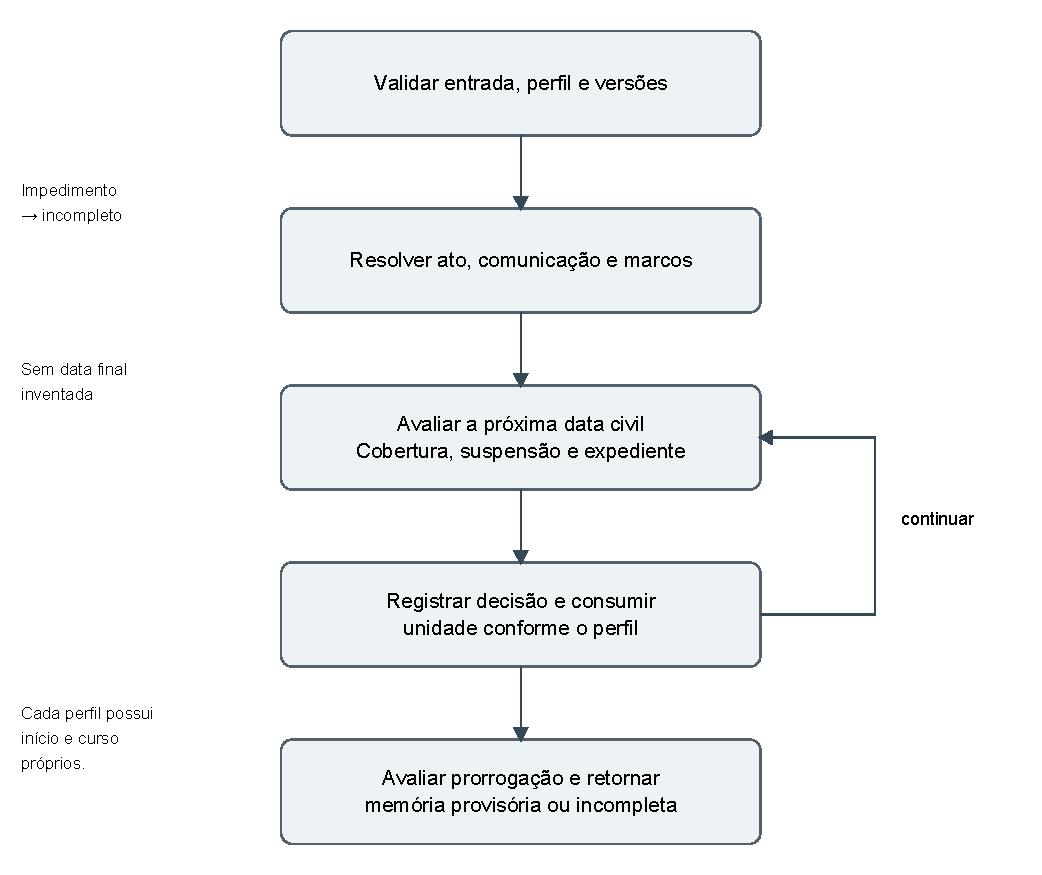
\includegraphics[width=\linewidth,height=.49\textheight,keepaspectratio]{figuras/calculo.pdf}
\par\smallskip{\fontsize{10}{12}\selectfont Fonte: elaboração para este relatório a partir do código e da documentação do Prazo Claro (2026).}
\end{figure}
O pseudocódigo descreve a organização, e não substitui as diferenças internas dos perfis:

\begin{quote}\begin{singlespace}\raggedright\ttfamily\footnotesize
\hspace*{0.0em}validar entrada e selecionar versões compatíveis\\
\hspace*{0.0em}se ato informado: verificar condições e duração\\
\hspace*{0.0em}determinar comunicação e marco inicial do perfil\\
\hspace*{0.0em}para cada data civil necessária:\\
\hspace*{2.0em}se cobertura/condição insuficiente: retornar incompleto\\
\hspace*{2.0em}avaliar início, suspensão, expediente e contagem\\
\hspace*{2.0em}registrar data, motivos, fontes e ordinal aplicável\\
\hspace*{2.0em}consumir unidade somente quando o perfil determinar\\
\hspace*{0.0em}se houver fim nominal: avaliar prorrogação própria\\
\hspace*{0.0em}retornar memória com versões, avisos e vencimento possível\\
\end{singlespace}\end{quote}
O motor civil 0.2.0 foi preservado. Os perfis ordinários criminal e trabalhista utilizam 0.3.0; a camada de composição de atos identifica 0.4.0 e informa também a versão da contagem delegada. Uma alteração de catálogo não reescreve uma versão anterior. Na travessia trabalhista, a aplicação tenta inicialmente o calendário anual existente e compõe 2026--2027 somente quando o percurso alcança o fim da cobertura e os componentes são compatíveis e contíguos.

Publicação, contagem e prorrogação não usam um único predicado genérico de dia útil. Um dia sem expediente e uma suspensão do curso do prazo podem produzir efeitos diferentes conforme a fase. A composição recusa lacunas, sobreposição, composição aninhada e eventos duplicados. Quando a informação não permite continuar, o sistema mantém dueDate nulo e informa as pendências em todos os formatos.

\section{Memória, exportação e histórico}
\label{section-5-3}
A memória contém entrada normalizada, evento, publicação, início, primeiro dia computado, fim nominal quando aplicável, vencimento, trilha, fontes e metadados. snapshot.calendar preserva cobertura e eventos; snapshot.rule e snapshot.act aparecem conforme o perfil. Componentes anuais ficam identificados quando há composição. O JSON e a impressão conservam os avisos demonstrativos.

Salvar no histórico envia a entrada e o título opcional ao servidor, que calcula novamente sob os catálogos internos. Não se aceita um vencimento do navegador como autoridade. Na leitura, o original é validado estruturalmente e permanece separado da recomputação. Quando a versão necessária não pode ser reexecutada, recomputed permanece nulo e o usuário conserva acesso ao original legível.

Paginação e filtro são aplicados com proprietário fixo, ordem por created\_at e id e tamanho limitado. A exclusão atualiza os totais da interface e trata a última página esvaziada. Títulos devem ser fictícios na demonstração, porque o campo livre pode conter dados que o sistema não precisa para contar.

\section{Conta e autenticação}
\label{section-5-4}
E-mail e senha, convite, recuperação e Google foram integrados ao Supabase Auth. Cadastro e recuperação usam confirmação por mensagem e retorno controlado. A troca PKCE utiliza o mesmo contexto de navegador para validar o retorno. O indicador de conectado permite perceber a sessão, e os recursos privados continuam verificando identidade em cada operação relevante.

\begin{figure}[H]\centering
\caption{Confirmação de cadastro e criação de sessão}
\label{figure-6}
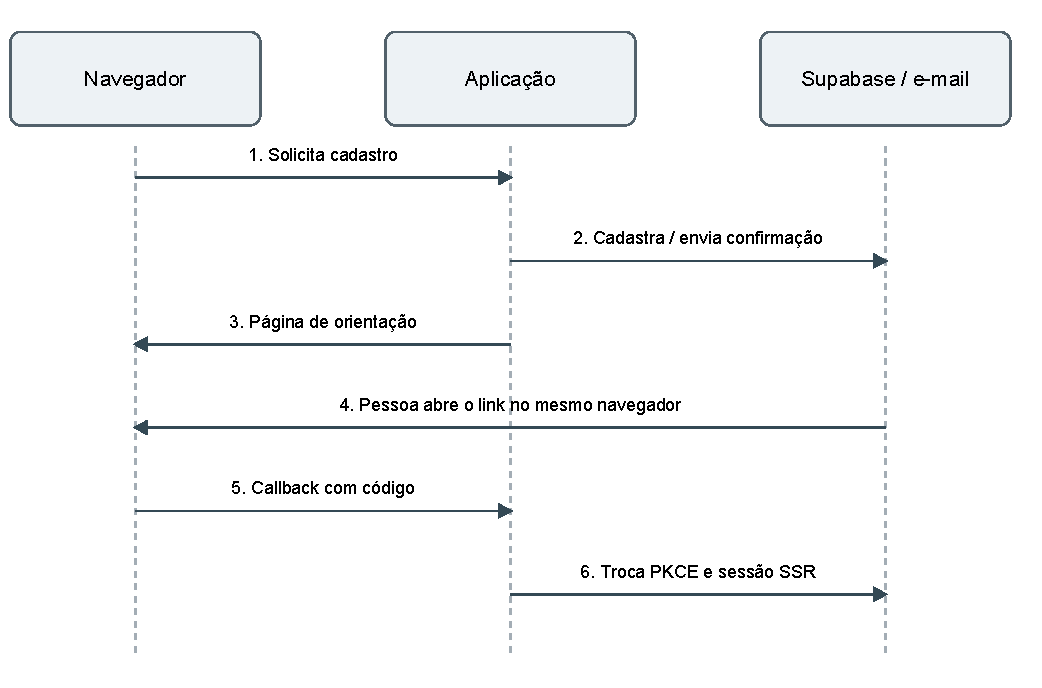
\includegraphics[width=\linewidth,height=.49\textheight,keepaspectratio]{figuras/autenticacao.pdf}
\par\smallskip{\fontsize{10}{12}\selectfont Fonte: elaboração para este relatório a partir do código e da documentação do Prazo Claro (2026).}
\end{figure}
A configuração de Site URL e de destinos permitidos no Supabase participa do retorno dos e-mails. Ela é diferente das URLs autorizadas no cliente Google. Os templates locais do CLI também não atualizam automaticamente o projeto hospedado. Essa distinção foi registrada durante a integração, pois receber a mensagem, abrir o destino e obter uma sessão são etapas diferentes.

\section{Lembretes e concorrência}
\label{section-5-5}
O lembrete é opcional e associado a um cálculo salvo elegível. A pessoa escolhe zero, um ou três dias corridos de antecedência e 09h, 12h ou 18h no fuso de São Paulo. Essa antecedência não altera a contagem processual. O destino é o e-mail confirmado atual do proprietário; o navegador não escolhe outro destinatário. No modo Brevo, há consentimento específico para envio externo.

Os modos local e Brevo são persistidos e isolados. Migrations não promovem registros antigos para envio real. Claim com token e bloqueio de linhas concorrentes permite reservar trabalho; a preparação revalida as condições imediatamente antes do envio. O dispatcher limita tentativas e trata resultados ambíguos de forma conservadora.

\begin{figure}[H]\centering
\caption{Estados principais de uma geração de lembrete}
\label{figure-7}
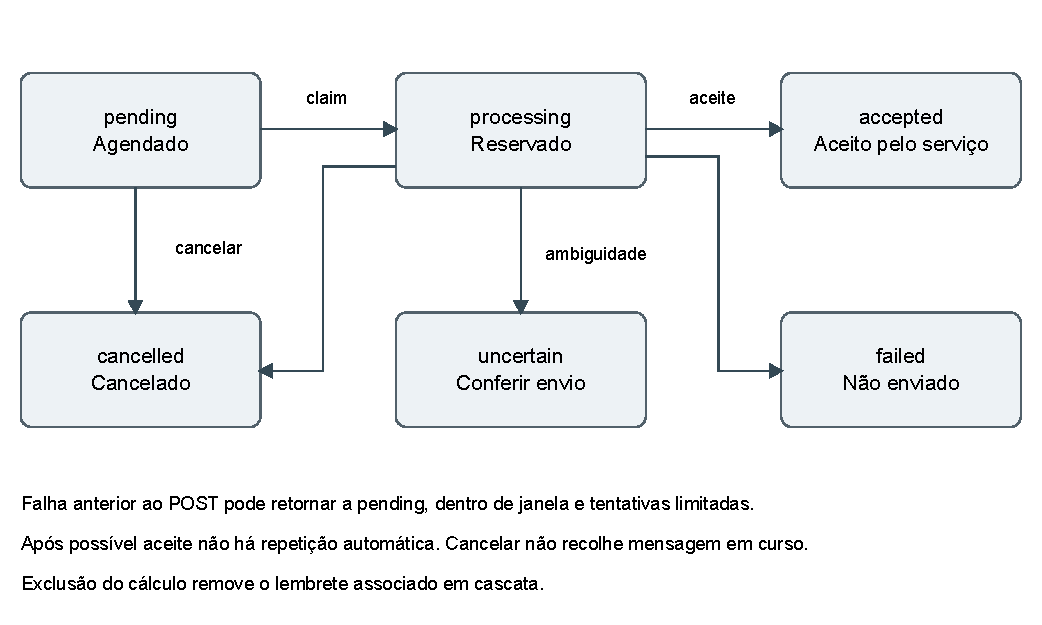
\includegraphics[width=\linewidth,height=.49\textheight,keepaspectratio]{figuras/lembretes.pdf}
\par\smallskip{\fontsize{10}{12}\selectfont Fonte: elaboração para este relatório a partir do código e da documentação do Prazo Claro (2026).}
\end{figure}
O estado accepted significa que o provedor aceitou a mensagem. Não demonstra recebimento, leitura ou execução do ato processual. Timeout ou resposta ambígua após iniciar o POST pode produzir uncertain, sem repetição automática que arrisque duplicação. Cancelamento não recolhe uma mensagem já aceita. As transições e as diferenças entre falha anterior ao envio e resposta incerta possuem testes SQL e de aplicação.

O adaptador Brevo considera sucesso o aceite HTTP 201 com identificador válido, conforme o contrato do provedor \hyperref[ref:BREVO]{(BREVO, s.d.)}. SMTP de autenticação e API de lembretes usam configurações distintas. O conteúdo enviado é mínimo e aponta para a memória privada, cujo acesso continua dependendo da conta proprietária. Não existe e-mail imediato adicional de confirmação do agendamento: a confirmação aparece no site, e a mensagem é prevista para o horário escolhido.

\section{Agendamento e implantação}
\label{section-5-6}
Supabase Cron consulta periodicamente o trabalho elegível e pg\_net chama o dispatcher hospedado. A chamada leva assinatura temporária, operação, timestamp e nonce de uso único. O segredo permanente fica no Vault e no servidor; não é copiado para cabeçalhos persistidos da fila HTTP. O servidor consome a invocação antes de executar. Probe verifica configuração sem obter lembretes nem enviar mensagens.

\begin{figure}[H]\centering
\caption{Implantação e processamento hospedado}
\label{figure-8}
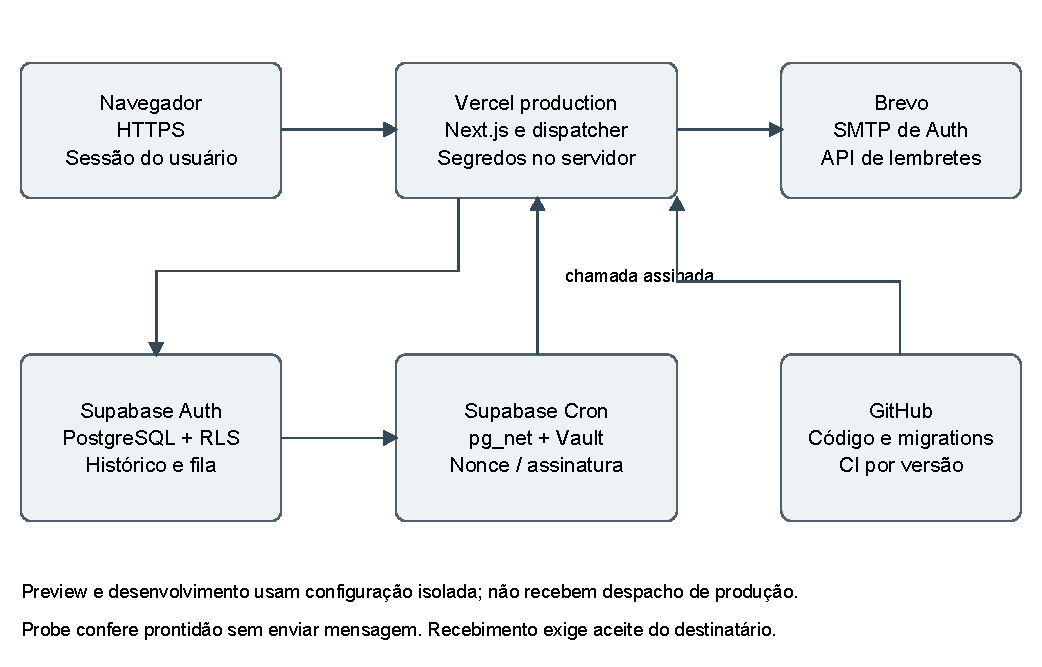
\includegraphics[width=\linewidth,height=.49\textheight,keepaspectratio]{figuras/implantacao.pdf}
\par\smallskip{\fontsize{10}{12}\selectfont Fonte: elaboração para este relatório a partir do código e da documentação do Prazo Claro (2026).}
\end{figure}
A configuração separa desenvolvimento, preview e produção. O preview não recebe credenciais de despacho do banco de produção. O job é preparado inativo; ativação exige diagnóstico recente e pronto. A suspensão operacional combina desativar o agendador e a entrega no servidor. A interface de lembrete informa seu estado sem depender de manter o navegador aberto no processamento hospedado.

A publicação funcional identificada ficou READY na Vercel no domínio https://tg-kezia2.vercel.app. O pacote fonte é gerado por commit, com manifesto e SHA-256, sem .git, dependências, builds ou .env privados. O pacote não contém contas ou dados e não substitui backup do Supabase. Operação ampliada depende de definir responsáveis e exercitar restauração, limites e atendimento.

\section{Estratégia e execução dos testes}
\label{section-5-7}
Os testes unitários verificam marcos, exclusões, travessias, versões, condições de atos e respostas incompletas. Os testes de propriedades exploram invariantes, sem substituir os casos jurídicos de referência. Os testes SQL verificam RLS, proprietário, modos de entrega, concorrência e transições. Os testes de navegador verificam formulário, navegação, exportação e apresentação de estados; alguns usam respostas controladas de API.

Integrações reais locais complementam as simulações: duas contas e acesso anônimo exercitam isolamento; Mailpit permite confirmar e recuperar conta e observar um lembrete sem enviar a terceiros. Os helpers usam identidades efêmeras e limpeza. A política de não reutilizar usuários reais de produção evita transformar um teste automatizado em alteração de dados pessoais.

No caso da página após cadastro, o primeiro teste falhou porque a navegação continuava em /entrar. Depois da implementação, os cenários desktop e celular passaram. Houve ainda uma falha intermediária de seletor de teste, documentada e corrigida sem ser apresentada como defeito do produto. Essa sequência distingue correção de implementação de ajuste do instrumento de verificação.
